\documentclass[document.tex]{subfiles}
\begin{document}
	
\chapter{Introduction}

\section{Overview}
\noindent Hyperspectral sensors simultaneously measure hundreds of continuous spectral bands with a fine resolution to form a three dimensional hyperspectral image data cube. For instance, the AVIRIS sensor simultaneously measures 224 bands with a fine resolution of 0.01$\mu$m. This high data volume presents many challenges which creates opportunity for research. The data captured are highly correlated and contains a significant amount of redundant data. All the image bands are not equally important for specific application.  Also, as the feature space dimension increases, if the size of the training data does not grow correspondingly, a reduction in the classification accuracy of the testing data is observed due to poor parameter estimation of the supervised classifier. This effect is known as the Hughes phenomenon. So it is required to extract only relevant features from the input dataset. Therefore an effective and efficient technique to find this relevant features is a major interest in current literature. Principal component analysis (PCA) is one of the most popular feature extraction technique, though its components is not always suitable for better classification accuracy. It is also not sensitive to input classes and consider only the global variance of the dataset. There are few techniques for finding relevant features in current literature. For example, mutual information based feature selection and in combination of principal component analysis and normalized mutual information based feature selection. A target class oriented feature selection technique is proposed as an alternative for the effective subspace detection in collaboration with kernel support vector machine (SVM) to achieve better classification accuracy.

\clearpage  

\section{Remote Sensing}
\noindent Remote sensing is the acquisition of information about an object or phenomenon without making physical contact with the object. Remote sensing is used in numerous fields, including geography, land surveying and most Earth Science disciplines (for example, hydrology, ecology, oceanography, glaciology, geology); it also has military, intelligence, commercial, economic, planning, and humanitarian applications.
\begin{figure}[H]
	\begin{center}
		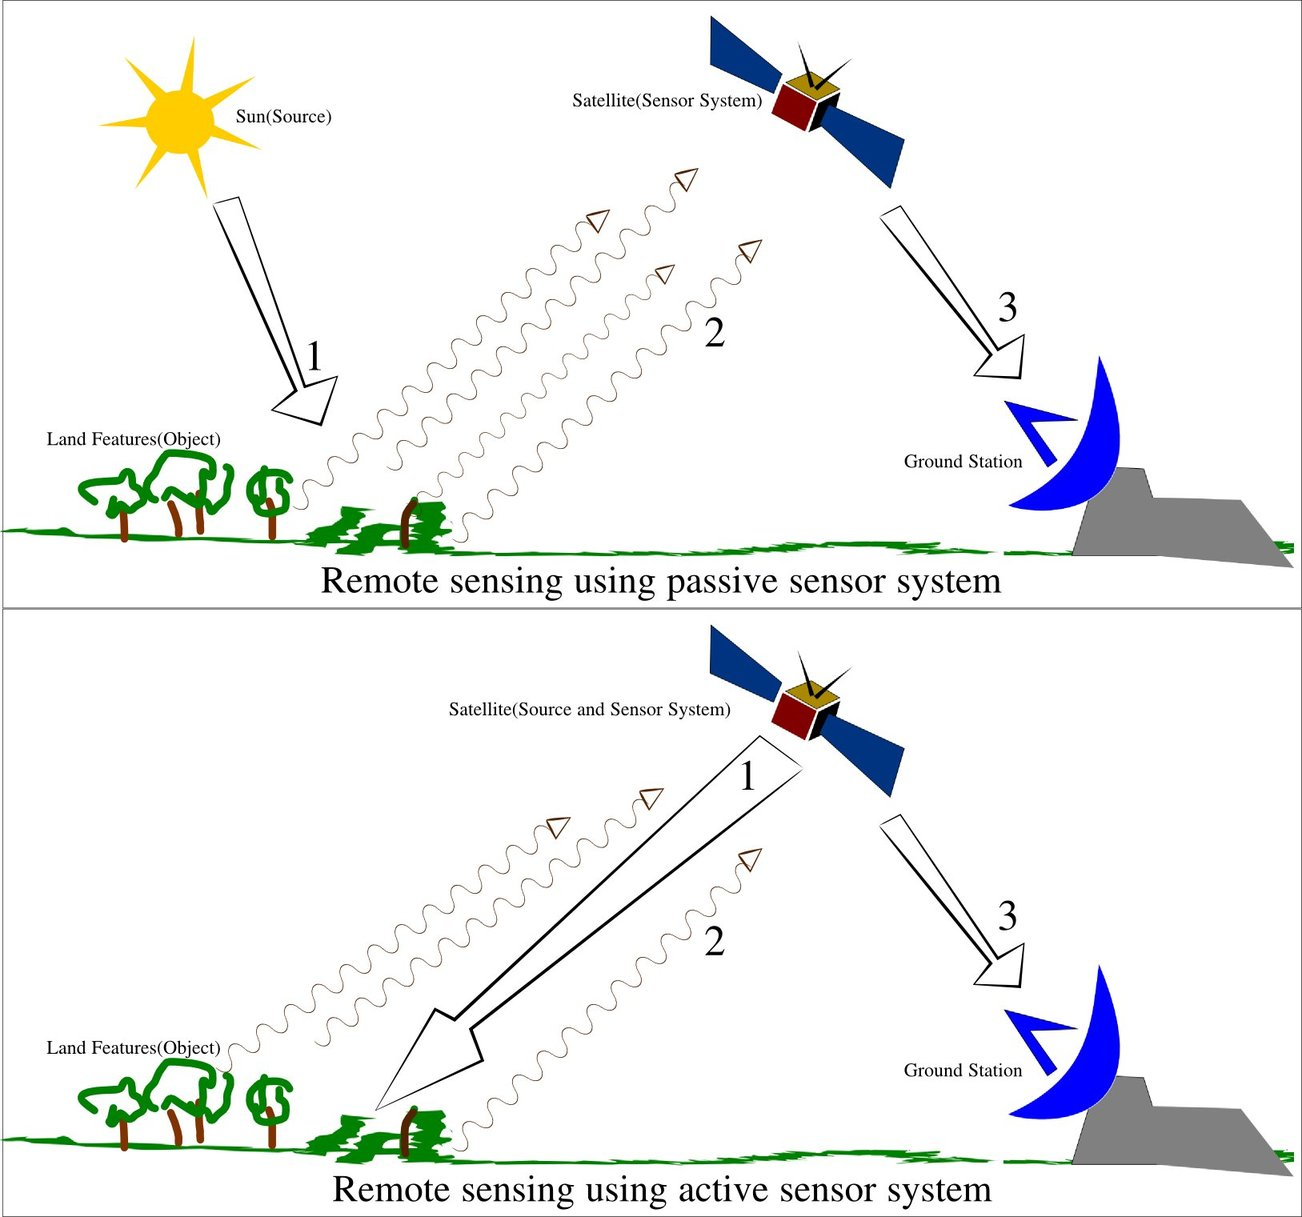
\includegraphics[height=8.0cm]{imgs/Remote_Sensing.jpg}
	\end{center}
	\caption{Remote Sensing}
	\label{fig: Remote Sensing}
\end{figure}
\noindent In current usage, the term "remote sensing" generally refers to the use of satellite- or aircraft-based sensor technologies to detect and classify objects on Earth, including on the surface and in the atmosphere and oceans, based on propagated signals (e.g. electromagnetic radiation). It may be split into "active" remote sensing (i.e., when a signal is emitted by a satellite or aircraft and its reflection by the object is detected by the sensor) and "passive" remote sensing (i.e., when the reflection of sunlight is detected by the sensor).

\section{Challenges of Remote Sensing Data}
\noindent Hyperspectral imaging is a popular field of remote sensing. The main challenge of hyperspectral image is its highly correlated huge data set. On the other hand, this large number of spectral bands has a direct impact on the required computational cost for classification. Also, as the
feature space dimension increases, if the size of the training data does not grow correspondingly, a reduction in the classification accuracy of the testing data is observed due to poor parameter estimation of the supervised classifier. This effect is known as the Hughes phenomenon\cite{1}.
\begin{figure}[H]
	\begin{center}
		\includegraphics[height=6.0cm]{imgs/curse.png}
	\end{center}
	\caption{Curse of dimensionality}
	\label{fig: Curse of dimensionality}
\end{figure}

\section{Motivation}
\noindent Hyperspectral image processing is fast growing research field because of its various application. Observed area of hyperspectral images are classified into different groups of object by classification of the image. Feature extraction and selecting only relevant features before classification is an important task to achieve high classification accuracy\cite{3}. So relevant feature selection is very important for classification of hyperspectral images. 

\section{Objectives}
\noindent The main goal of this research is to illustrate a target class oriented feature mining method which is a combination of feature extraction and feature selection which gives a better classification accuracy. 

Objective of this research will be:
\begin{itemize}
	\item Create a method of feature extraction by removing correlation among bands.
	\item Create an approach to select features after feature extraction.
	\item Create a method with collaboration of feature mining and classification.
	\item Improving classification accuracy.
\end{itemize}

\section{Organization}
\noindent This report is organized in 5 chapters discussing all related topics that may be helpful in reproducing a feature selection method for hyperspectral image classification.\\
Chapter 1\\
A short overview of the whole research field and topic is discussed in this chapters.\\
Chapter 2\\
Chapter 3\\
Chapter 4\\
Chapter 5\\
 
\end{document}
